\newpage
\chapter{Manual de usuario}
Como se ha podido ver en la descripción de la solución propuesta y en su implementación, se han creado dos aplicaciones de cara al usuario: una aplicación de administración y una aplicación móvil para el usuario final. En esta sección se va a realizar un recorrido por estas dos aplicaciones explicando al usuario cómo funcionan.
\section{Aplicación de administración}
La aplicación de administración está creada para que los usuarios provenientes de la Administración Pública y la autoridad puedan gestionar el sistema vía web. Esta gestión es: administrar las plazas de aparcamiento y las acreditaciones para aparcar en este tipo de plazas, así como recibir alertas de plazas que estén siendo mal usadas.
\\\\
En todas las pantallas de la aplicación aparecen notificaciones cuando un vehículo sin acreditación ocupa un aparcamiento. Estas notificaciones se actualizan cada 15 segundos y al pulsar sobre ellas van a dirigir al usuario a la pantalla de gestión de plazas. A continuación se puede ver un ejemplo de estas notificaciones:
%\begin{figure}[H]
%	\centering
%	\includegraphics[width=0.9\textwidth]{imagenes/administracion/alerta.png}
%	\caption{Vista principal: ejemplo alerta plaza mal ocupada}
%	\label{administración_alerta}
%\end{figure}
%La pantalla que se muestra anteriormente es la principal de la aplicación donde el usuario puede acceder a las diversas secciones de la misma: gestión de plazas, ubicaciones o acreditaciones; como se puede ver en la figura \ref{administración_alerta}. Aquí el administrador puede elegir qué gestionar. 

\subsection{Gestión de ubicaciones de aparcamiento}
Si el administrador quiere gestionar las ubicaciones de aparcamiento del sistema, debería acceder a ``Ubicaciones''. Estas son donde existen las plazas de aparcamiento monitorizadas.
\begin{figure}[H]
	\centering
	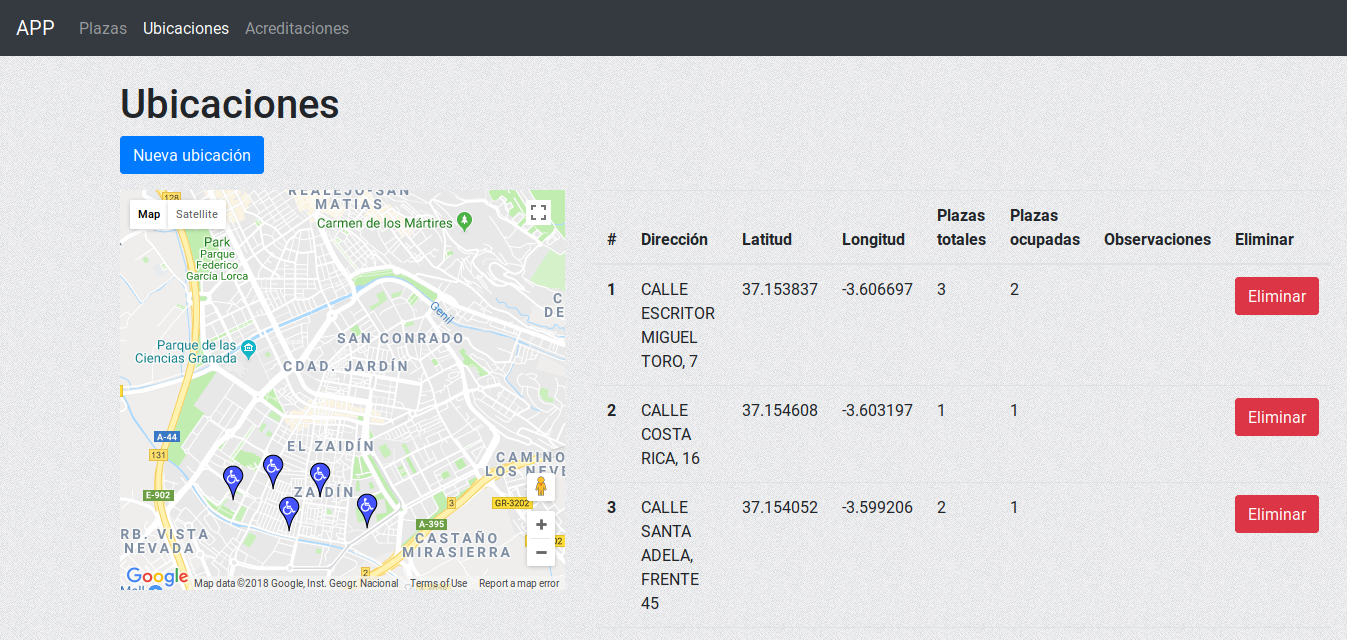
\includegraphics[width=0.9\textwidth]{imagenes/administracion/ubicaciones.png}
	\caption{Vista de ubicaciones: aplicación de administración}
	\label{administracion_ubicaciones}
\end{figure}
En esta sección, figura \ref{administracion_ubicaciones}, se pueden ver las distintas ubicaciones existentes en el sistema, ya sea posicionadas en el mapa o en la lista con más detalles como su dirección, coordenadas GPS, número de plazas u observaciones. Este pantalla se actualiza automáticamente para que su información sea en tiempo real ya que el número de plazas ocupadas podría cambiar. También da la posibilidad de añadir una nueva ubicación, figura \ref{administracion_ubicaciones_nueva}, donde hay que administrarle una posición GPS a mano o pinchando la posición en el mapa y una dirección. Las observaciones no son obligatorias.
\begin{figure}[H]
	\centering
	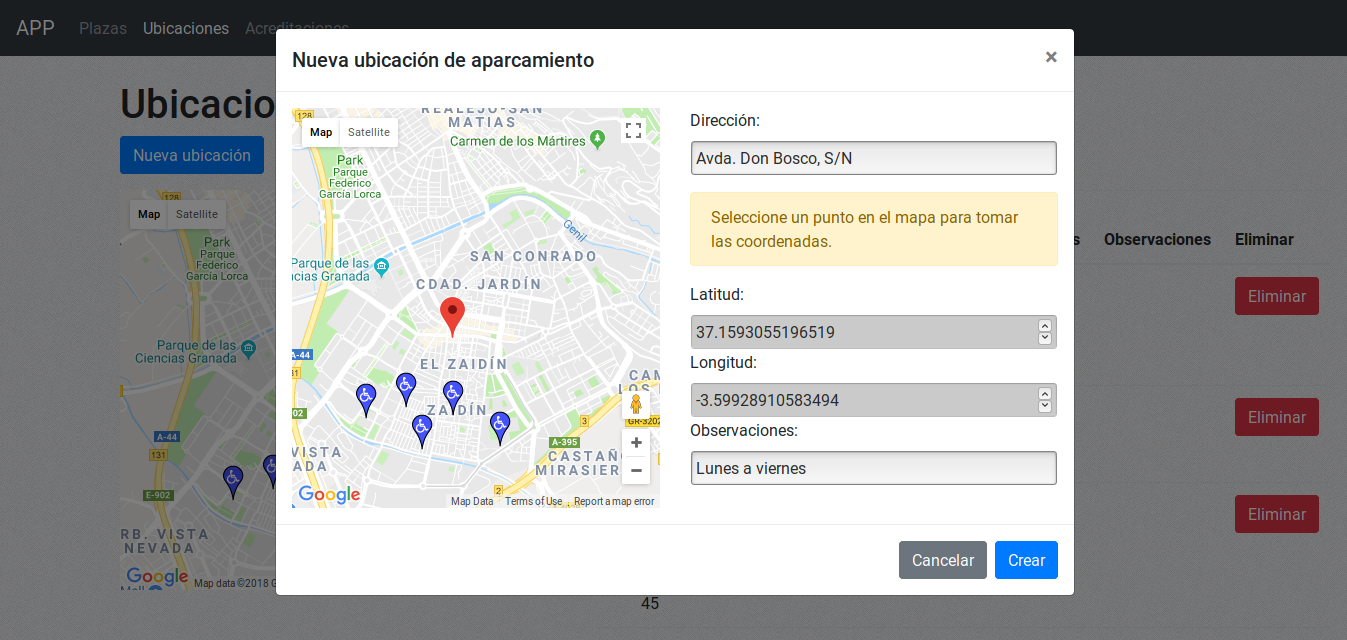
\includegraphics[width=0.9\textwidth]{imagenes/administracion/ubicaciones_nueva.png}
	\caption{Vista de creación de una nueva ubicación: aplicación de administración}
	\label{administracion_ubicaciones_nueva}
\end{figure}
Si no se indica ni la dirección ni las coordenadas de la ubicación, la aplicación advierte con un mensaje de error indicando que se necesita rellenar los datos obligatorios para dar de alta una nueva ubicación, figura \ref{administracion_ubicacion_nueva_error}.
\begin{figure}[H]
	\centering
	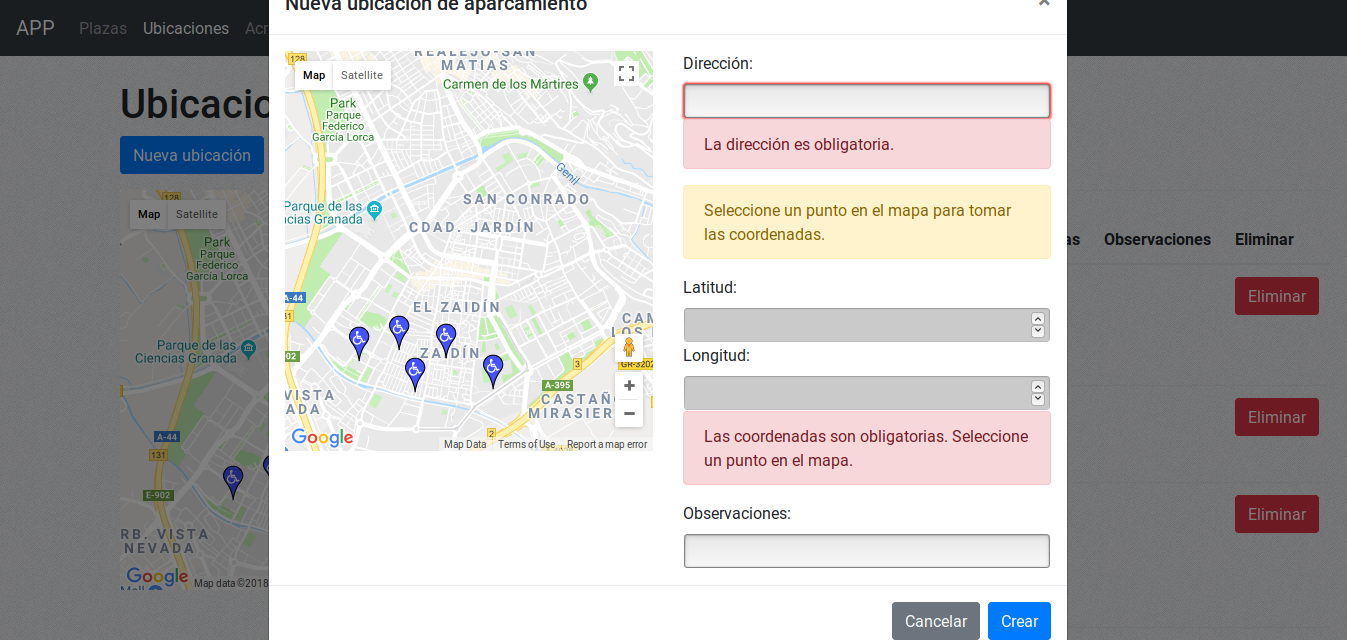
\includegraphics[width=0.9\textwidth]{imagenes/administracion/ubicaciones_nueva_error.png}
	\caption{Vista de error en la creación de una nueva ubicación: aplicación de administración}
	\label{administracion_ubicacion_nueva_error}
\end{figure}
Si se indican correctamente los datos para crear una nueva ubicación, el sistema añadirá la nueva ubicación, figura \ref{administracion_ubicaciones_creada}.
\begin{figure}[H]
	\centering
	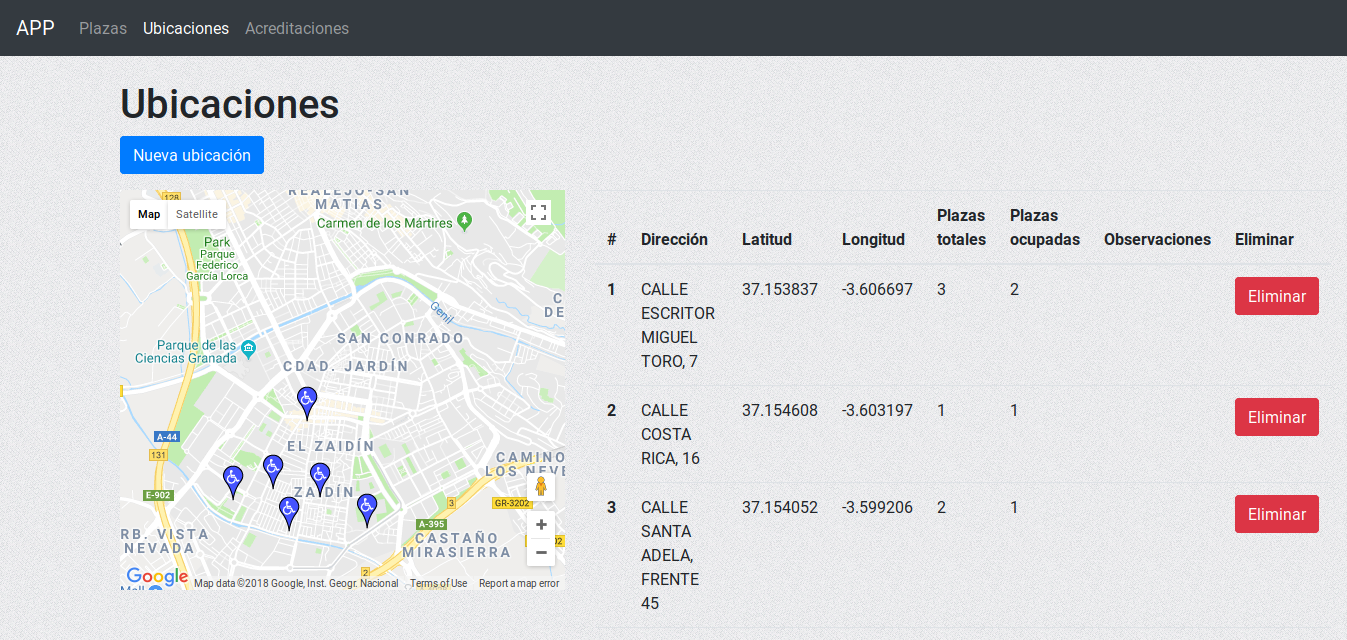
\includegraphics[width=0.9\textwidth]{imagenes/administracion/ubicaciones_creada.png}
	\caption{Vista listado con nueva ubicación: aplicación de administración}
	\label{administracion_ubicaciones_creada}
\end{figure}
En esta pantalla, junto al listado de las ubicaciones existentes, la aplicación permite eliminar de forma fácil una ubicación del sistema siempre y cuando no tenga plazas asociadas, figura \ref{administracion_ubicaciones_eliminar}.
\begin{figure}[H]
	\centering
	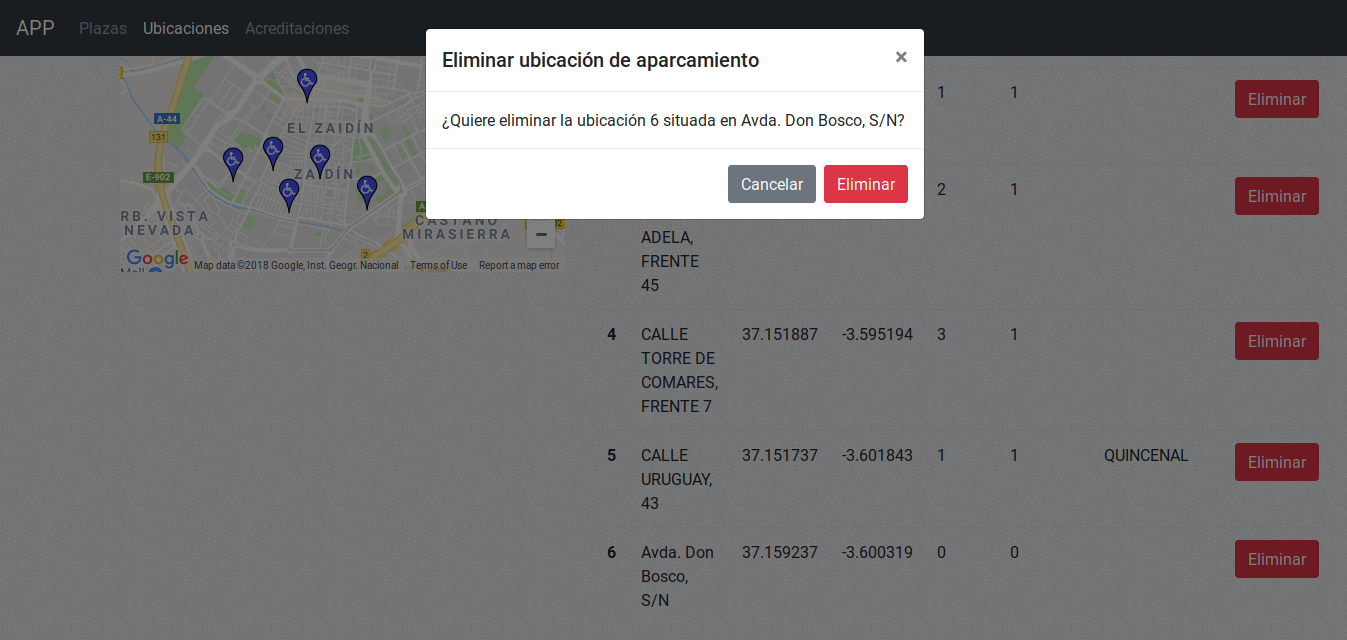
\includegraphics[width=0.9\textwidth]{imagenes/administracion/ubicaciones_eliminar.png}
	\caption{Vista de eliminación de una ubicación: aplicación de administración}
	\label{administracion_ubicaciones_eliminar}
\end{figure}
Si la ubicación que se quiere eliminar tiene plazas asociadas, no se podrá realizar la acción. Si se trata de eliminar, la aplicación muestra el siguiente mensaje de error:
\begin{figure}[H]
	\centering
	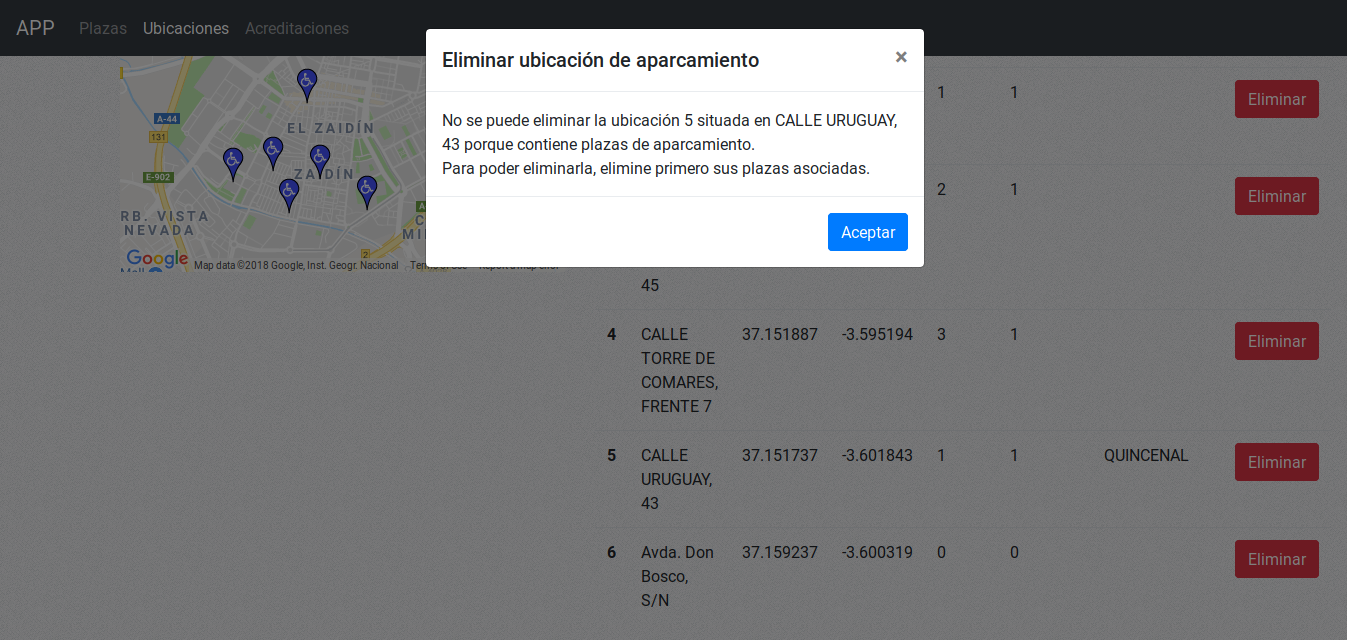
\includegraphics[width=0.9\textwidth]{imagenes/administracion/ubicaciones_eliminar_error.png}
	\caption{Vista de error en la eliminación de una ubicación: aplicación de administración}
	\label{administracion_ubicaciones_eliminar_error}
\end{figure}

\subsection{Gestión de plazas de aparcamiento}
Si el administrador quiere gestionar las plazas de aparcamiento del sistema, debería acceder a ``Plazas''. Estas son monitorizadas y tienen que estar en una ubicación a la que pertenece.
\begin{figure}[H]
	\centering
	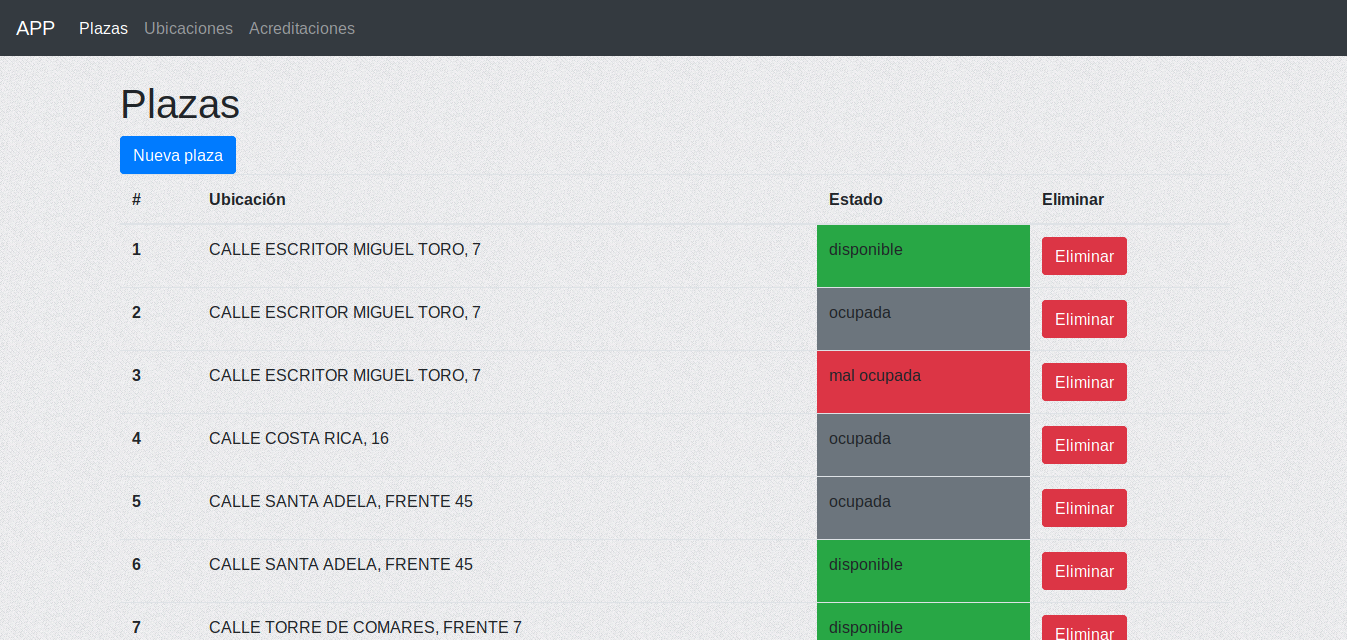
\includegraphics[width=0.9\textwidth]{imagenes/administracion/plazas.png}
	\caption{Vista de plazas: aplicación de administración}
	\label{administracion_plazas}
\end{figure}
En esta sección, figura \ref{administracion_plazas}, se pueden ver las distintas plazas existentes en el sistema junto a su estado actual: plaza disponible, ocupado o mal ocupado. Este pantalla se actualiza automáticamente para que su información sea en tiempo real. También da la posibilidad de añadir una nueva plaza, figura \ref{administracion_plazas_nueva}, donde hay que seleccionar aquella ubicación donde se quiere añadir la nueva plaza.
\begin{figure}[H]
	\centering
	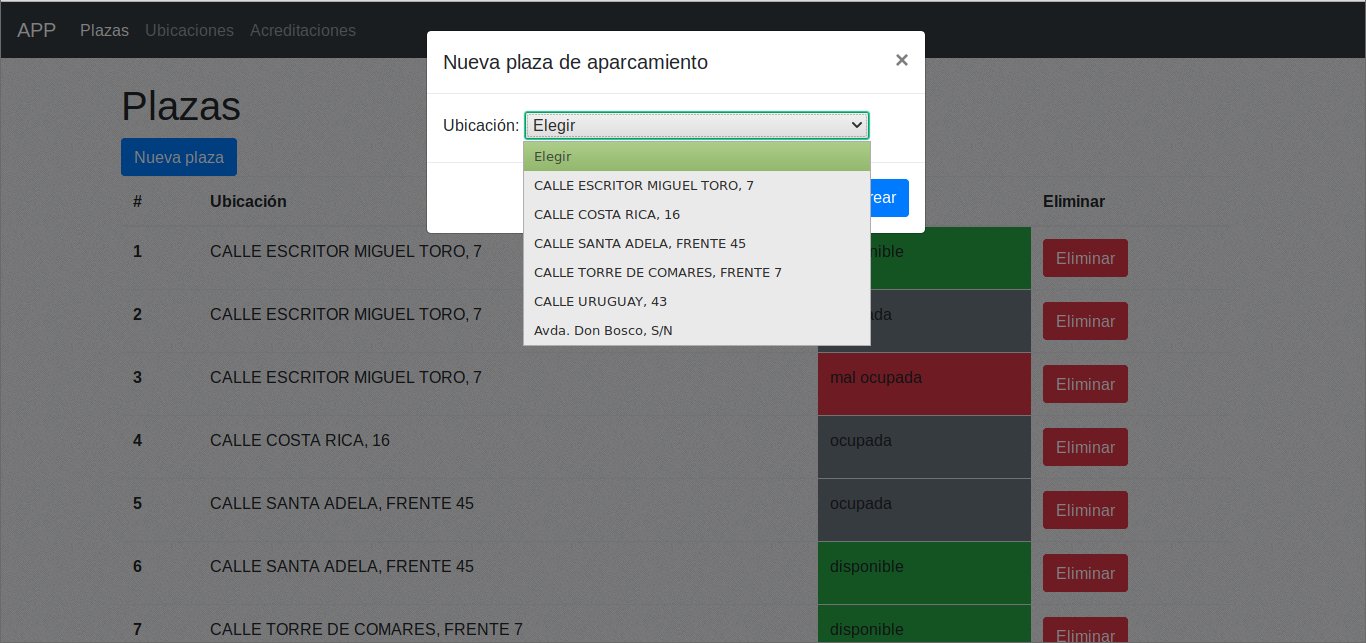
\includegraphics[width=0.9\textwidth]{imagenes/administracion/plazas_nueva.png}
	\caption{Vista de creación de una nueva plaza: aplicación de administración}
	\label{administracion_plazas_nueva}
\end{figure}
Si no se indica dicha ubicación, la aplicación advierte con un mensaje de error indicando que se necesita seleccionar una ubicación, figura \ref{administracion_plazas_nueva_error}.
\begin{figure}[H]
	\centering
	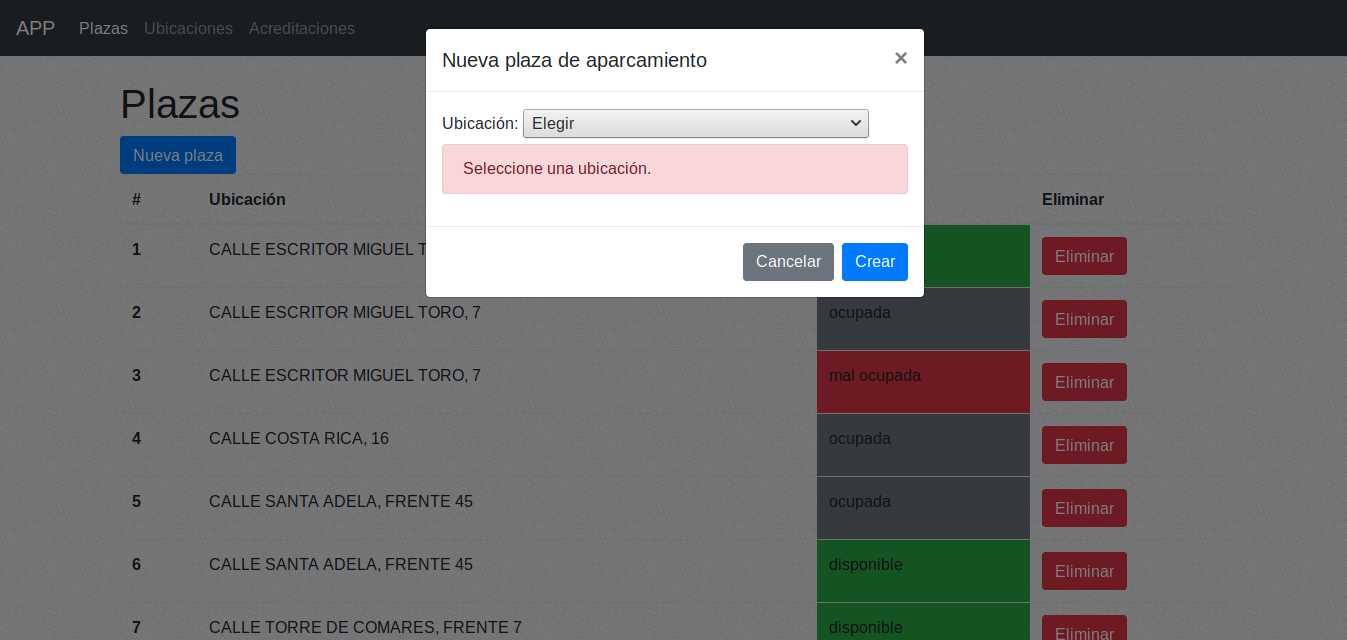
\includegraphics[width=0.9\textwidth]{imagenes/administracion/plazas_nueva_error.png}
	\caption{Vista de error en la creación de una nueva plaza: aplicación de administración}
	\label{administracion_plazas_nueva_error}
\end{figure}
Si se selecciona una ubicación, el sistema creará la nueva plaza, figura \ref{administracion_plazas_creada}.
\begin{figure}[H]
	\centering
	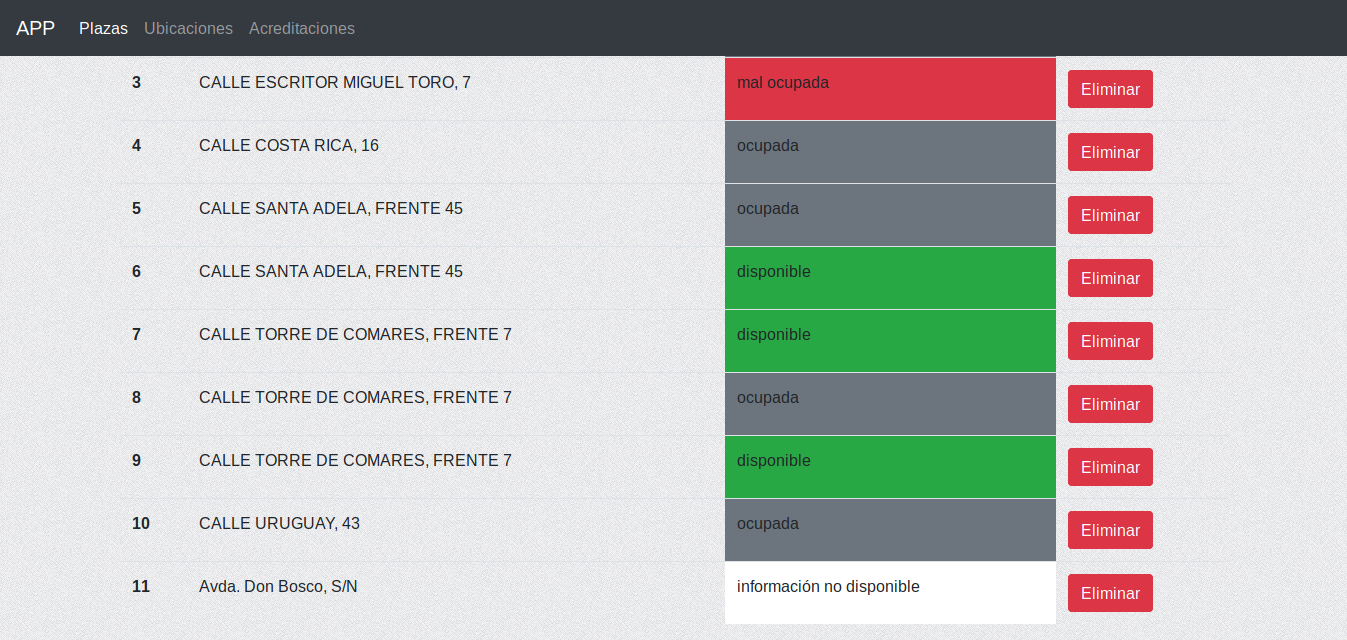
\includegraphics[width=0.9\textwidth]{imagenes/administracion/plazas_creada.png}
	\caption{Vista listado con nueva plaza: aplicación de administración}
	\label{administracion_plazas_creada}
\end{figure}
En esta pantalla, junto al listado de las plazas existentes, la aplicación permite eliminar de forma fácil una plaza del sistema, figura \ref{administracion_plazas_eliminar}.
\begin{figure}[H]
	\centering
	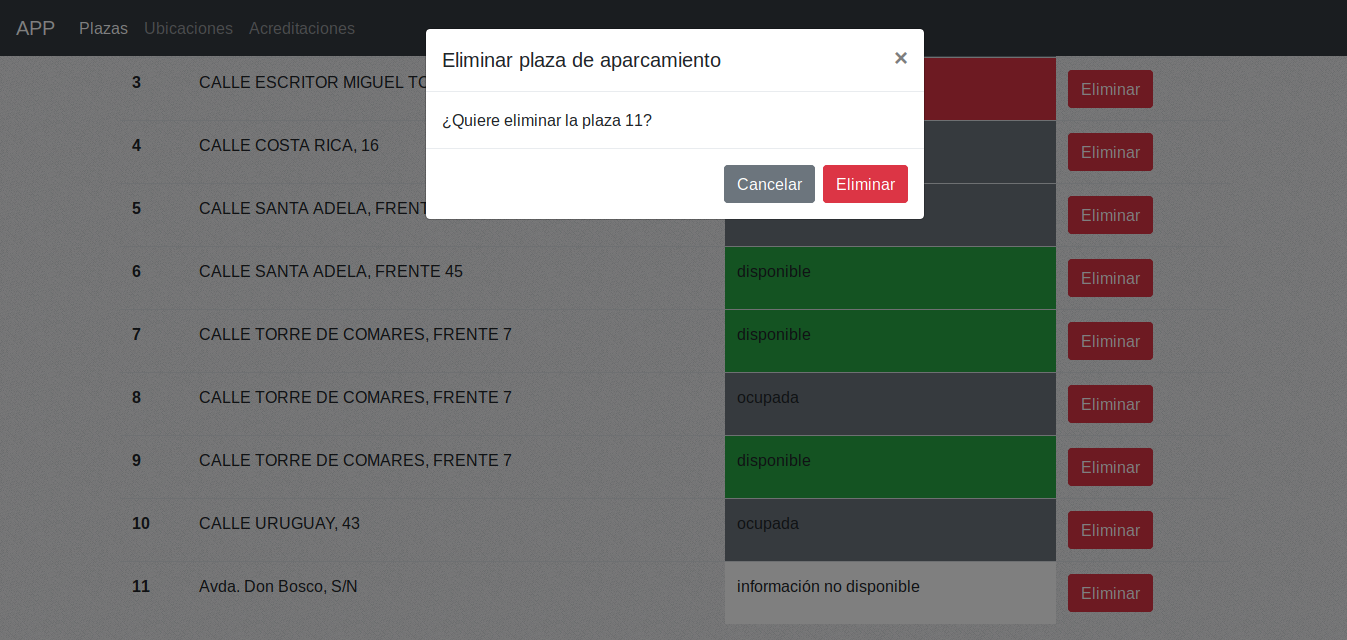
\includegraphics[width=0.9\textwidth]{imagenes/administracion/plazas_eliminar.png}
	\caption{Vista de eliminación de una plaza: aplicación de administración}
	\label{administracion_plazas_eliminar}
\end{figure}

\newpage
\subsection{Gestión de acreditaciones de aparcamiento}
Si el administrador quiere gestionar las acreditaciones de aparcamiento del sistema, debería acceder a ``acreditaciones''. Estas se ocupan de distinguir un vehículo con autorización que aparque lícitamente en una plaza reservada de uno que aparque ilícitamente.
\begin{figure}[H]
	\centering
	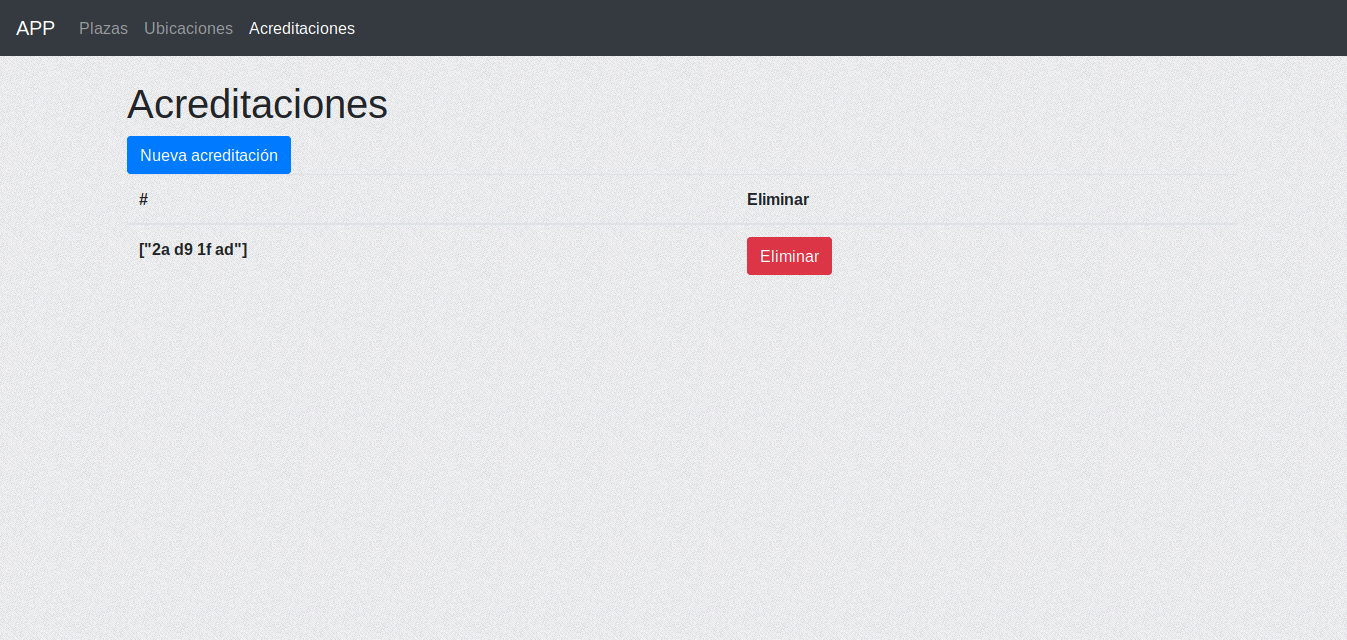
\includegraphics[width=0.9\textwidth]{imagenes/administracion/acreditaciones.png}
	\caption{Vista de acreditaciones: aplicación de administración}
	\label{administracion_acreditaciones}
\end{figure}
En esta sección, figura \ref{administracion_acreditaciones}, se pueden ver las distintas acreditaciones existentes en el sistema. Estas acreditaciones estarían vinculadas a una persona con movilidad reducida. También da la posibilidad de añadir una nueva ubicación, figura \ref{administracion_acreditaciones_nueva}, donde hay que administrarle un identificador inequívoco de la tarjeta de aparcamiento que dispone de un RFID.
\begin{figure}[H]
	\centering
	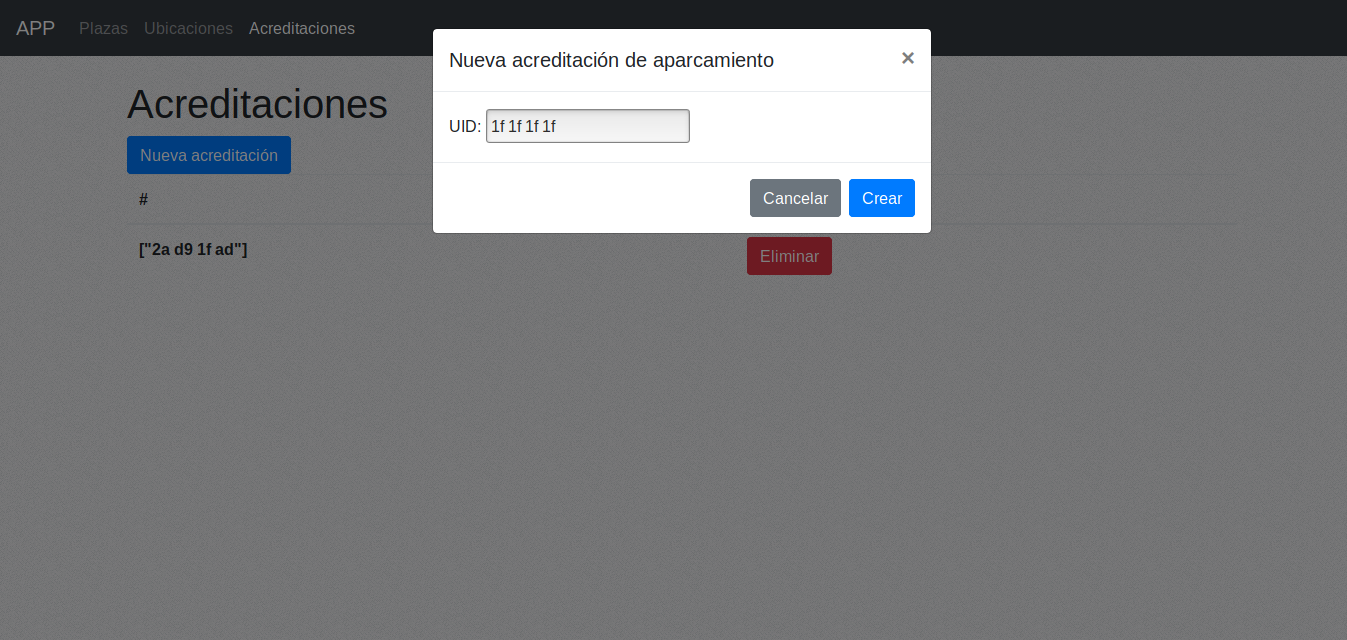
\includegraphics[width=0.9\textwidth]{imagenes/administracion/acreditaciones_nueva.png}
	\caption{Vista de creación de una nueva acreditación: aplicación de administración}
	\label{administracion_acreditaciones_nueva}
\end{figure}
Si no se indica dicho identificador, la aplicación advierte con un mensaje de error indicando que se necesita rellenar el dato obligatorio para dar de alta una nueva acreditación, figura \ref{administracion_acreditaciones_nueva_error}.
\begin{figure}[H]
	\centering
	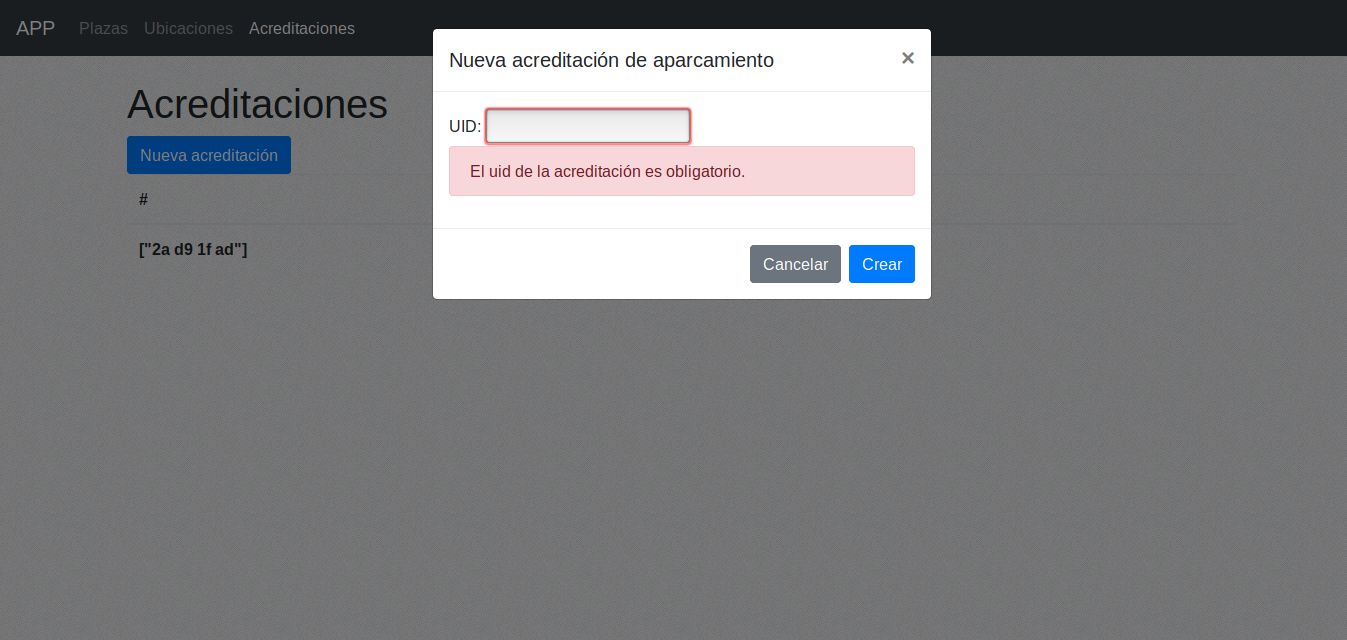
\includegraphics[width=0.9\textwidth]{imagenes/administracion/acreditaciones_nueva_error.png}
	\caption{Vista de error en la creación de una nueva acreditación: aplicación de administración}
	\label{administracion_acreditaciones_nueva_error}
\end{figure}
Si se indican correctamente el identificador para crear una nueva acreditación, el sistema añadirá la nueva acreditación, figura \ref{administracion_acreditaciones_creada}.
\begin{figure}[H]
	\centering
	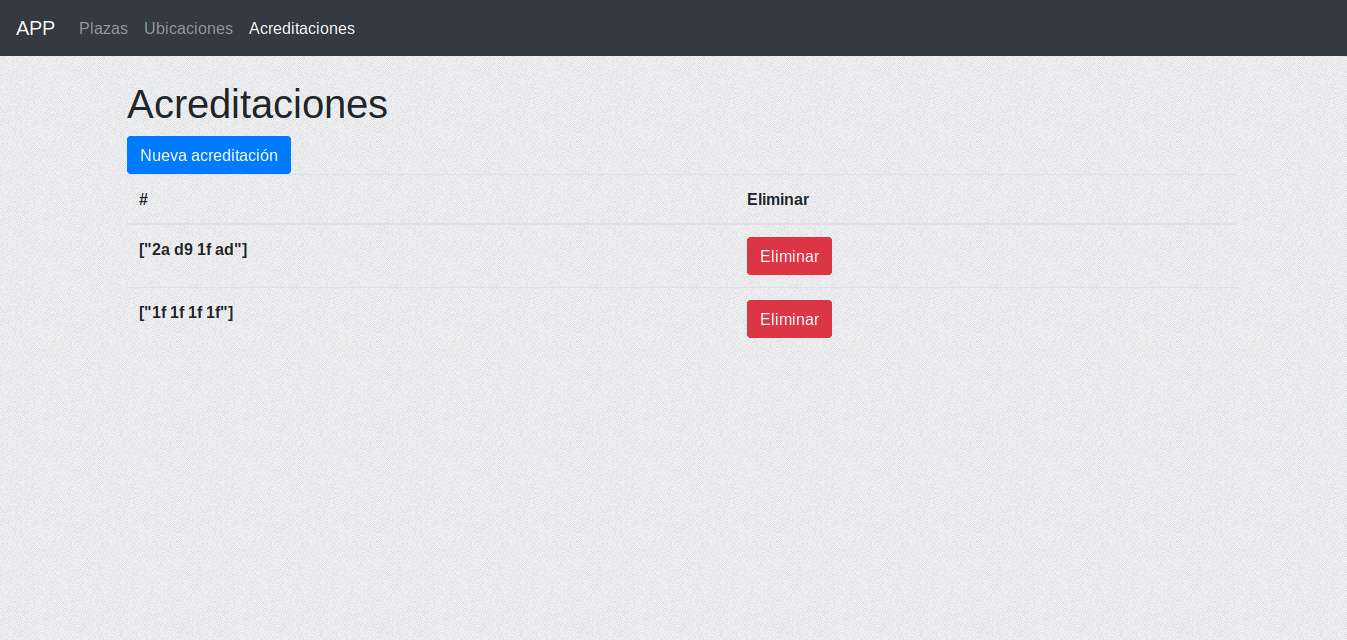
\includegraphics[width=0.9\textwidth]{imagenes/administracion/acreditaciones_creada.png}
	\caption{Vista listado con nueva acreditación: aplicación de administración}
	\label{administracion_acreditaciones_creada}
\end{figure}
En esta pantalla, junto al listado de las acreditaciones existentes, la aplicación permite eliminar de forma fácil una acreditación del sistema, figura \ref{administracion_acreditaciones_eliminar}.
\begin{figure}[H]
	\centering
	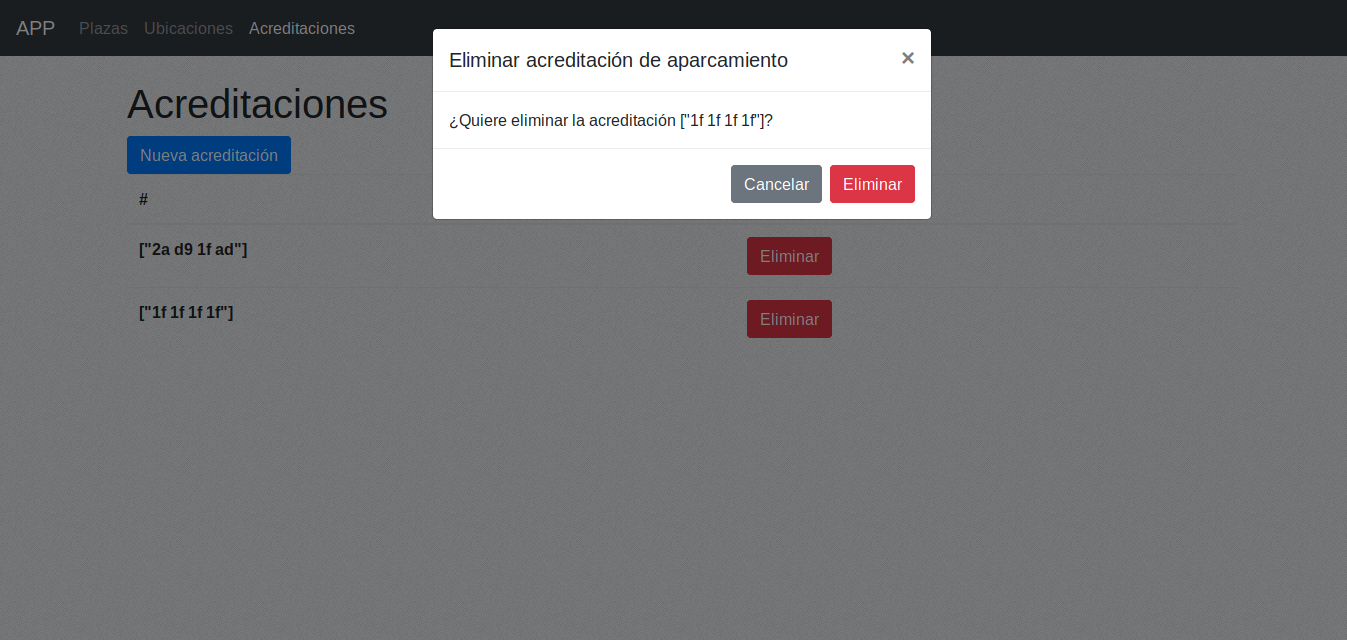
\includegraphics[width=0.9\textwidth]{imagenes/administracion/acreditaciones_eliminar.png}
	\caption{Vista de eliminación de una acreditación: aplicación de administración}
	\label{administracion_acreditaciones_eliminar}
\end{figure}

\newpage
\section{Aplicación de usuario}
La aplicación de usuario es una aplicación sencilla y amigable, diseñada para que el usuario desde su teléfono móvil, encuentre una plaza de aparcamiento cercana a su destino o se dirija a una plaza de aparcamiento que esté libre.
\begin{figure}[H]
	\centering
	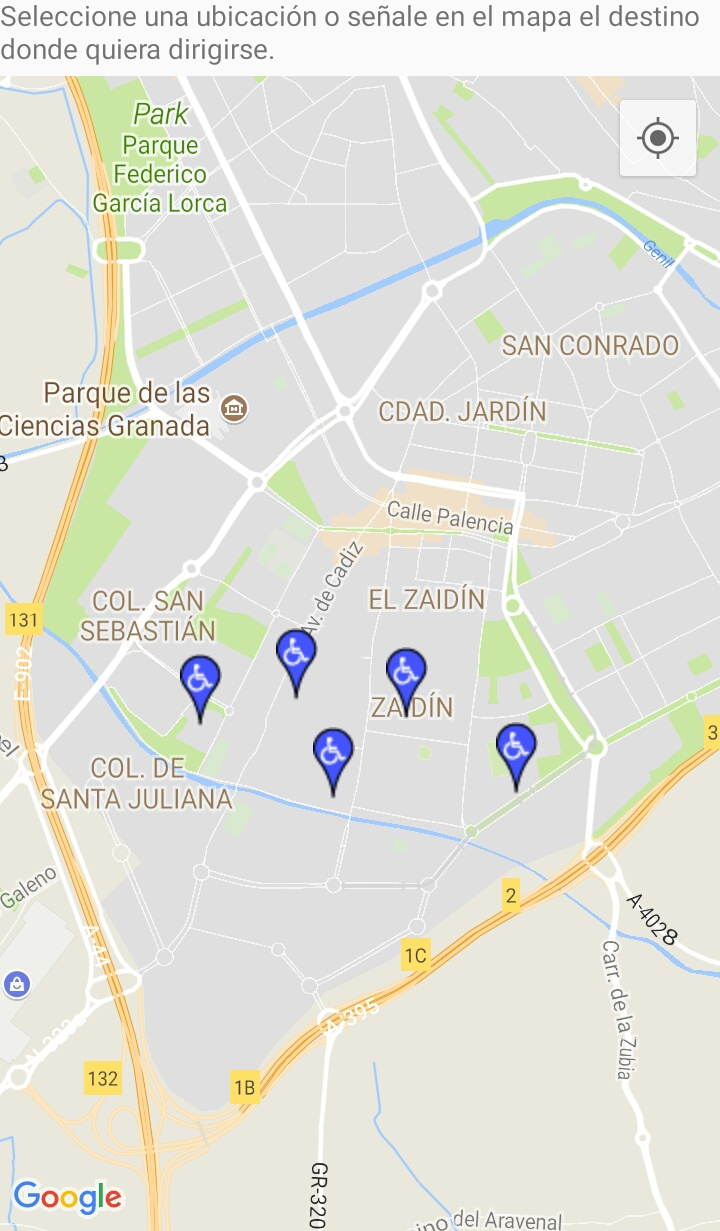
\includegraphics[width=0.4\textwidth]{imagenes/app/1.jpg}
	\caption{Vista inicial: aplicación de usuario}
	\label{app_1}
\end{figure}
Al abrir la aplicación, el usuario se encuentra un mapa donde se señalan las ubicaciones de aparcamiento, figura \ref{app_1}. Estas ubicaciones se van cargando a medida que el usuario se desplaza o amplia el mapa. Estas ubicaciones en forma de marcas en el mapa las puede señalar el usuario, apareciendo así una nueva ventana con información detallada sobre la ubicación, figura \ref{app_2}.
\begin{figure}[H]
	\centering
	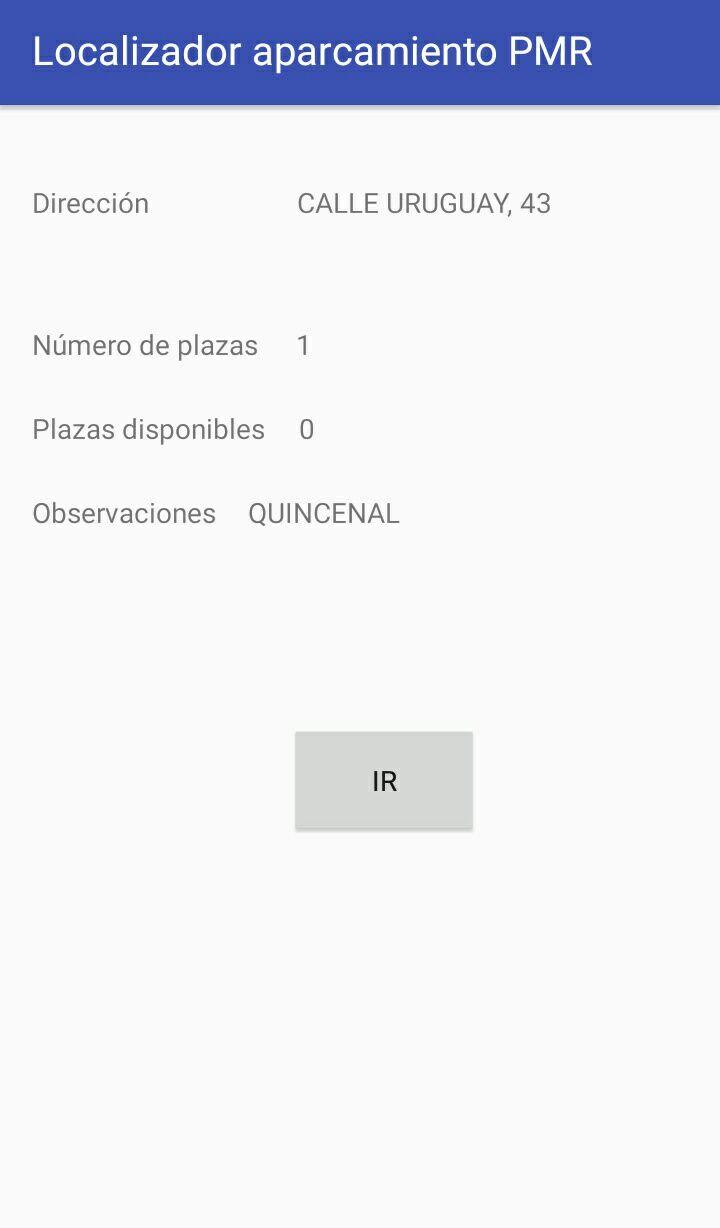
\includegraphics[width=0.4\textwidth]{imagenes/app/2.jpg}
	\caption{Vista detallada de ubicación: aplicación de usuario}
	\label{app_2}
\end{figure}
El usuario, si así lo desea, puede iniciar la navegación en automóvil hacia dicha ubicación pulsando el botón ``IR'', figura \ref{app_3}.
\begin{figure}[H]
	\centering
	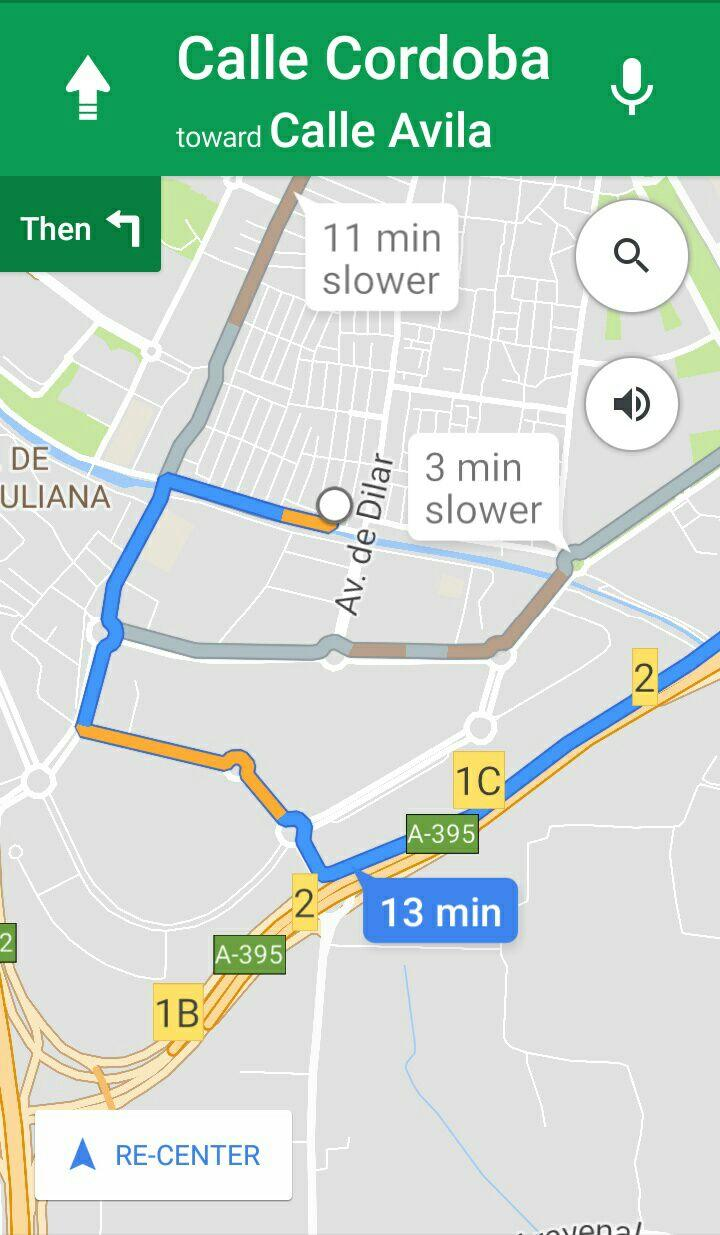
\includegraphics[width=0.4\textwidth]{imagenes/app/3.jpg}
	\caption{Vista navegación a ubicación: aplicación de usuario}
	\label{app_3}
\end{figure}
Desde el momento que inicia la navegación hasta que la finaliza, el usuario puede recibir una notificación indicándole, que la ubicación a la que se dirige, se ha quedado sin plazas libres. Dicha notificación sería:
\begin{figure}[H]
	\centering
	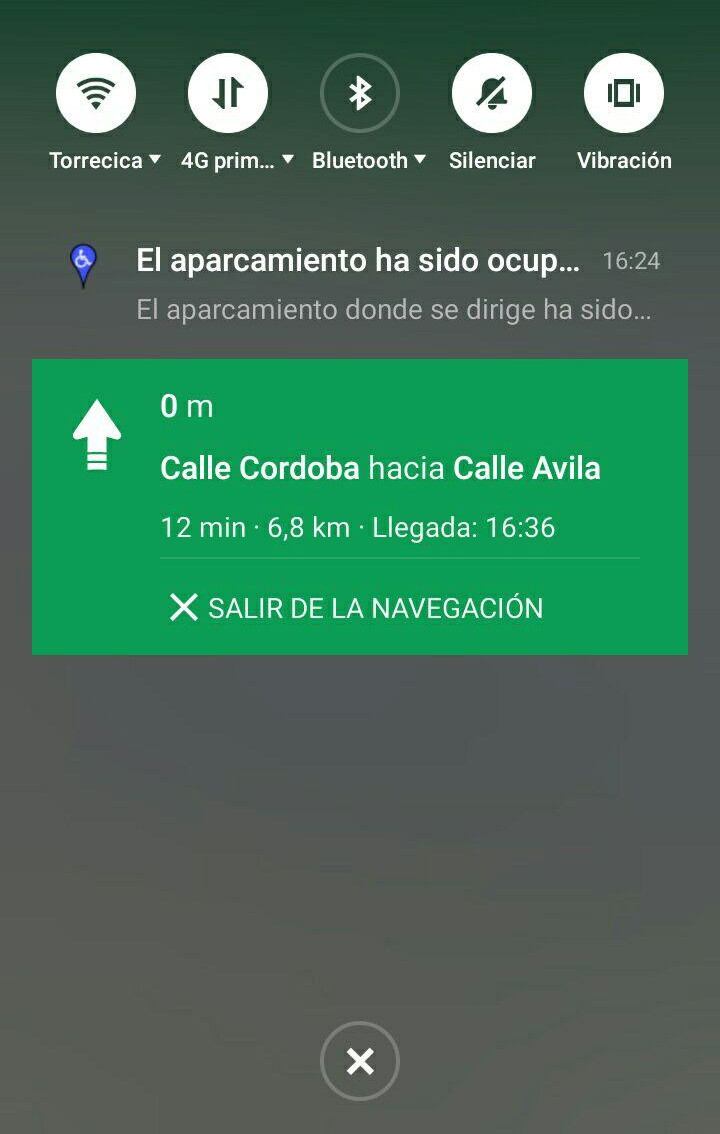
\includegraphics[width=0.4\textwidth]{imagenes/app/7.jpg}
	\caption{Vista notificación: aplicación de usuario}
	\label{app_7}
\end{figure}
Con respecto a la búsqueda de aparcamientos, el punto fuerte de esta aplicación es que el usuario puede introducir un destino pinchando en el mapa, figura \ref{app_4}.
\begin{figure}[H]
	\centering
	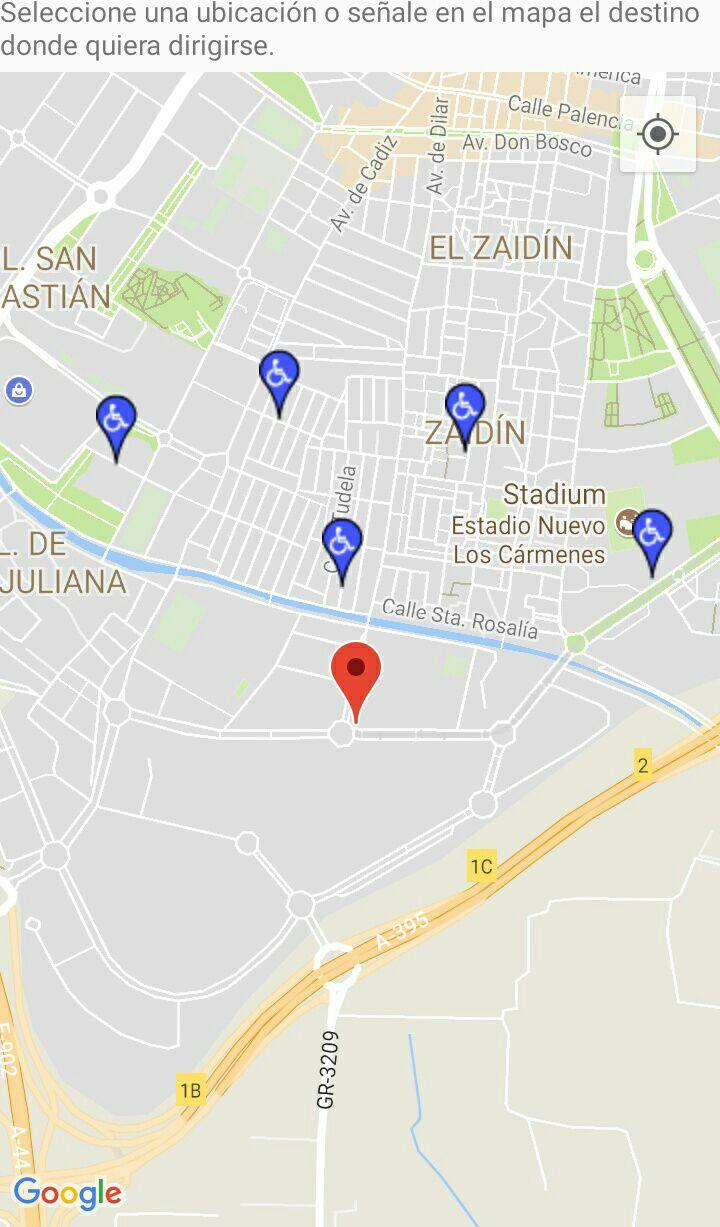
\includegraphics[width=0.4\textwidth]{imagenes/app/4.jpg}
	\caption{Vista creación de destino: aplicación de usuario}
	\label{app_4}
\end{figure}
En este momento, si el usuario mueve el mapa se borraría dicho destino. En cambie si vuelve a seleccionar su destino, la aplicación le muestra una lista de ubicaciones ordenadas por distancia al destino real del usuario donde poder aparcar, figura \ref{app_5}.
\begin{figure}[H]
	\centering
	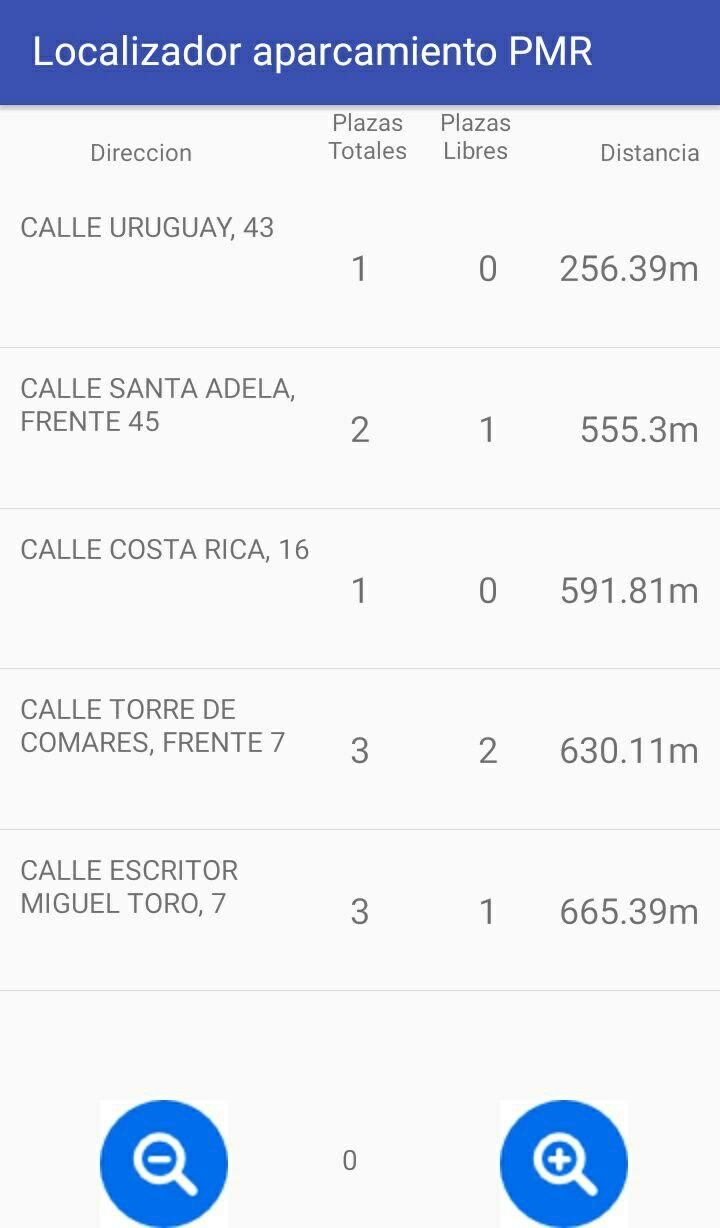
\includegraphics[width=0.4\textwidth]{imagenes/app/5.jpg}
	\caption{Vista listado de ubicaciones cercanas: aplicación de usuario}
	\label{app_5}
\end{figure}
En la lista se muestra la dirección de la plaza de aparcamiento cercana junto al número de aparcamientos que tiene, el número de ellos que están ocupados y la distancia al destino del usuario. Por otro lado, y si el usuario lo desea, puede reordenar la lista de manera que plazas más lejanas, con mayor número de aparcamientos libres, salgan en primeras posiciones. Por ello, en la parte inferior de la pantalla se han puesto dos botones de búsqueda.
\begin{figure}[H]
	\centering
	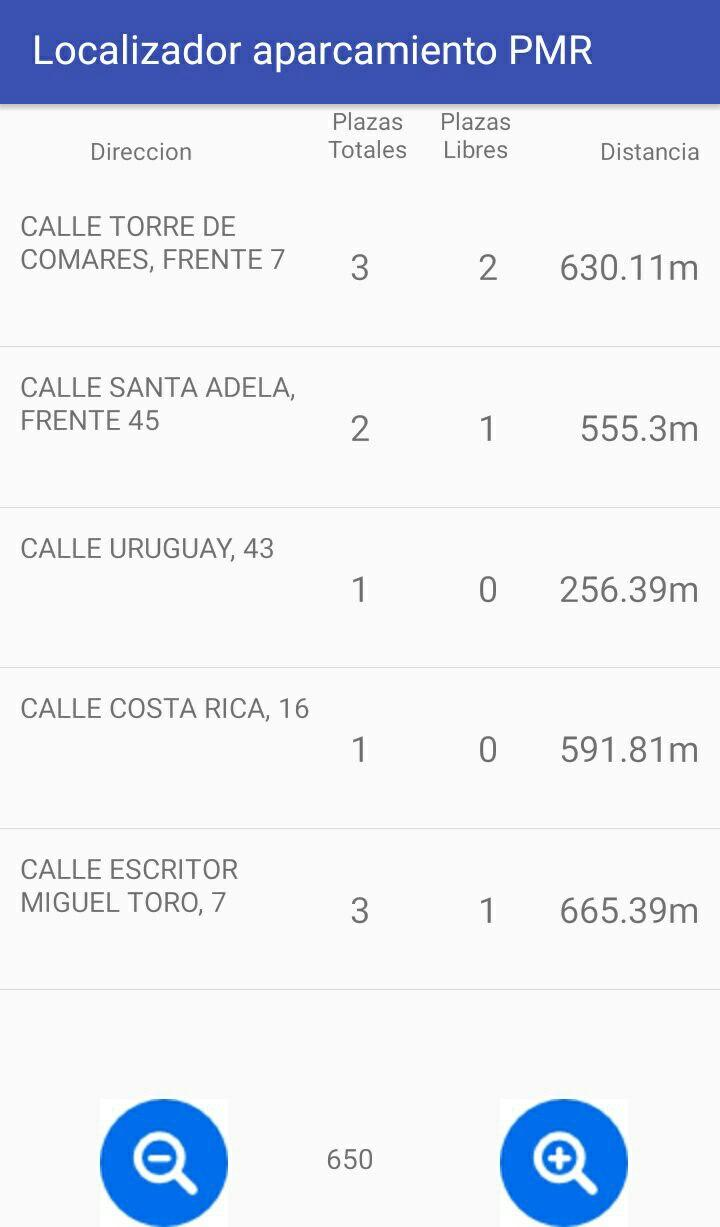
\includegraphics[width=0.4\textwidth]{imagenes/app/6.jpg}
	\caption{Vista listado de ubicaciones cercanas agrupado por distancias: aplicación de usuario}
	\label{app_6}
\end{figure}
Pulsando sobre el ``+'' la distancia que aparece entre los botones aumenta y las plazas se actualizan y ordenan. Es la  forma que tiene el usuario para decirle a la aplicación la distancia que estaría dispuesto a recorrer.
\\\\
Si el usuario selecciona un destino, la aplicación entraría en modo navegación al igual que anteriormente, figura \ref{app_3} haciendo uso de la aplicación Google Maps de Android.